\documentclass[]{article}
\usepackage{tikz}
\usepackage{pgf}
\usetikzlibrary{positioning}
\usetikzlibrary{shapes}
\usetikzlibrary{snakes}
\begin{document}

\section{Basic DAG}

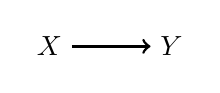
\begin{tikzpicture}
    % nodes %
    \node[text centered] (x) {$X$};
    \node[right = 1 of x, text centered] (y) {$Y$};
    % edges %
    \draw[->, line width = 1] (x) -- (y);
\end{tikzpicture}

\section{Simple Example DAG}

\begin{tikzpicture}
    % nodes %
    \node[text centered] (y) {$Y$};
    \node[right = 1 of x, text centered] (z) {$Z$};
    \node[above left = 1 of x, text centered] (u) {$U$};
    \node[below left = 1 of x, text centered] (x) {$X$};
    % edges %
    \draw[->, line width = 1] (y) -- (z);
    \draw[->, line width = 1] (x) -- (y);
    \draw[->, line width = 1] (u) -- (y);
\end{tikzpicture}

\section{Basic Confounder DAG}

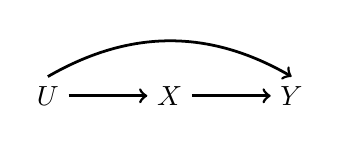
\begin{tikzpicture}
    % nodes %
    \node[text centered] (x) {$X$};
    \node[right = 1 of x, text centered] (y) {$Y$};
    \node[left = 1 of x, text centered] (u) {$U$};
    % edges %
    \draw[->, line width = 1] (x) -- (y);
    \draw[->, line width = 1] (u) -- (x);
    \draw[->, line width = 1] (u.north) [out=30,in=150] to (y.north);
\end{tikzpicture}

\section{Basic Selection DAG}
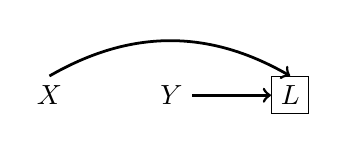
\begin{tikzpicture}
    % nodes %
    \node[text centered] (y) {$Y$};
    \node[right = 1 of y, text centered, rectangle, draw] (l) {$L$};
    \node[left = 1 of y, text centered] (x) {$X$};
    % edges %
    \draw[->, line width = 1] (y) -- (l);
    \draw[->, line width = 1] (x.north) [out=30,in=150] to (l.north);
\end{tikzpicture}


\end{document}

